\subsection{Itinerary Optimisation Algorithms}

We generated 50 random constraints and tested them out
on the PSO and GA algorithm. Figure~\ref{AverageScore} shows how the number of
particles affects the score. For 100 population
members, both algorithms achieve similar average
scores. However, the difference in score is not
proportional to the average time taken to complete a
single day, as shown in figure ~\ref{AverageTime}. Since other users will use
the application, we did not
want the generation's time to affect the user
experience. The difference between the average
score of 50 and 100 particles for PSO is only 0.5,
this variant provides the best balance of time and
score. Therefore it is the one chosen for our
application.   


\begin{figure}[h]
\centering
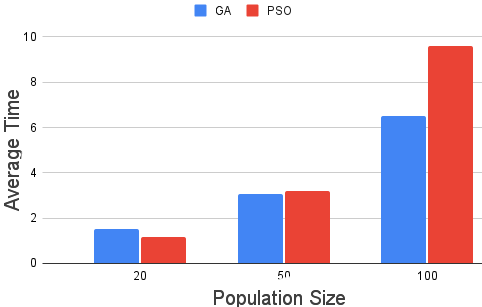
\includegraphics[width=0.3\textwidth]{AverageTime.png}
\caption{Average time spent for 50 iterations}
\label{AverageTime}
\end{figure}

\begin{figure}[h]
\centering
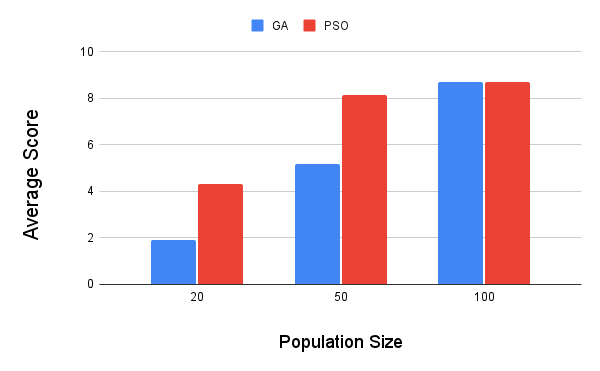
\includegraphics[width=0.3\textwidth]{AverageScore.png}
\caption{Average score achieved for 50 iterations}
\label{AverageScore}
\end{figure}
